\chapter{SYSTEM DESIGN}

\section{System Architecture}
The architecture follows the Model-View-Controller (MVC) paradigm natively supported by Laravel, combined with a progressive Single Page Application (SPA) frontend. By using Inertia.js, the backend seamlessly populates the React views without building a separate REST API, allowing secure traversal between the seller functionality and buyer browsing contexts.

\begin{figure}[H]
    \centering
    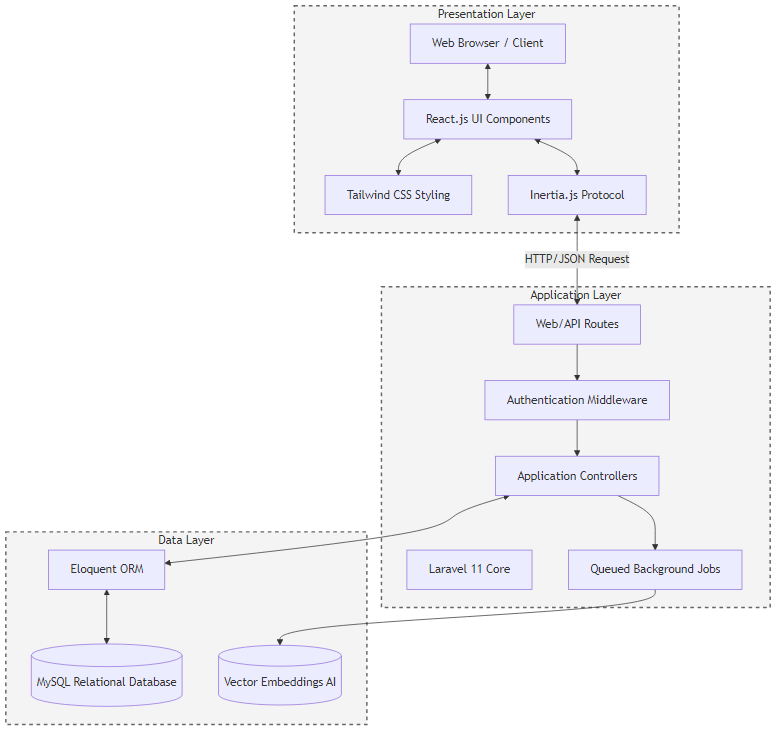
\includegraphics[width=0.8\textwidth]{architecture_diagram.png}
    \caption{System Architecture Diagram}
    \label{fig:architecture}
\end{figure}

\section{Use Case \& Activity Diagrams}
The core interactions of the system involve buyers discovering products and sellers managing inventory.
\\\\
\textbf{Use Case Diagram Explanation:} The Use Case diagram illustrates the division of capabilities. A standard Buyer can register, browse products using semantic search, add items to the cart, and proceed to checkout to receive a tracking ID. Conversely, the Seller role gains elevated access to the Seller Dashboard where they can authenticate, create new product listings, edit pricing, and fulfill pending orders.
\\\\
\textbf{Activity Diagram Explanation:} The Activity diagram traces the execution path from a user opening the platform to completing a purchase. It validates the session, maps the semantic embedding generation during product searches, triggers the secure checkout logic, and handles the subsequent redirection to the success page while dispatching background database updates.

\begin{figure}[H]
    \centering
    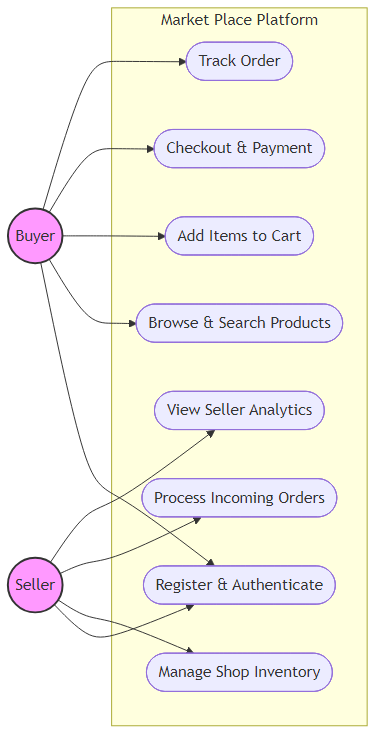
\includegraphics[width=0.8\textwidth]{use_case_diagram.png}
    \caption{Shopify Use Case Diagram}
    \label{fig:usecase}
\end{figure}

\begin{figure}[H]
    \centering
    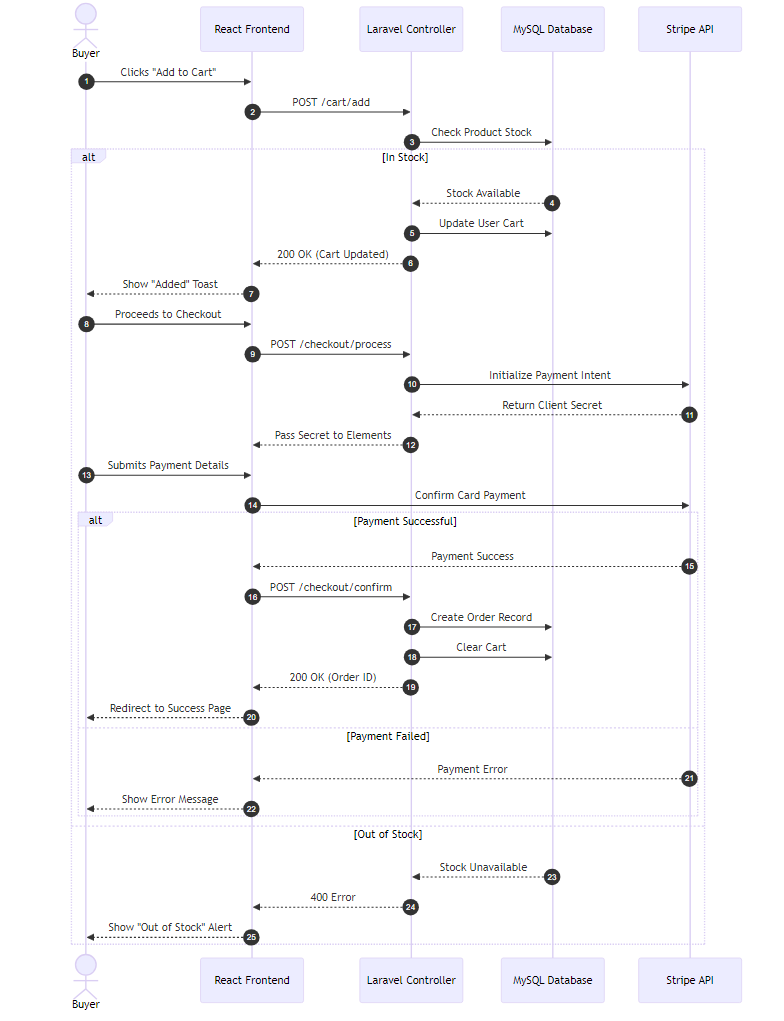
\includegraphics[width=0.8\textwidth]{sequence_diagram.png}
    \caption{Shopify Sequence Diagram}
    \label{fig:sequence}
\end{figure}

\begin{figure}[H]
    \centering
    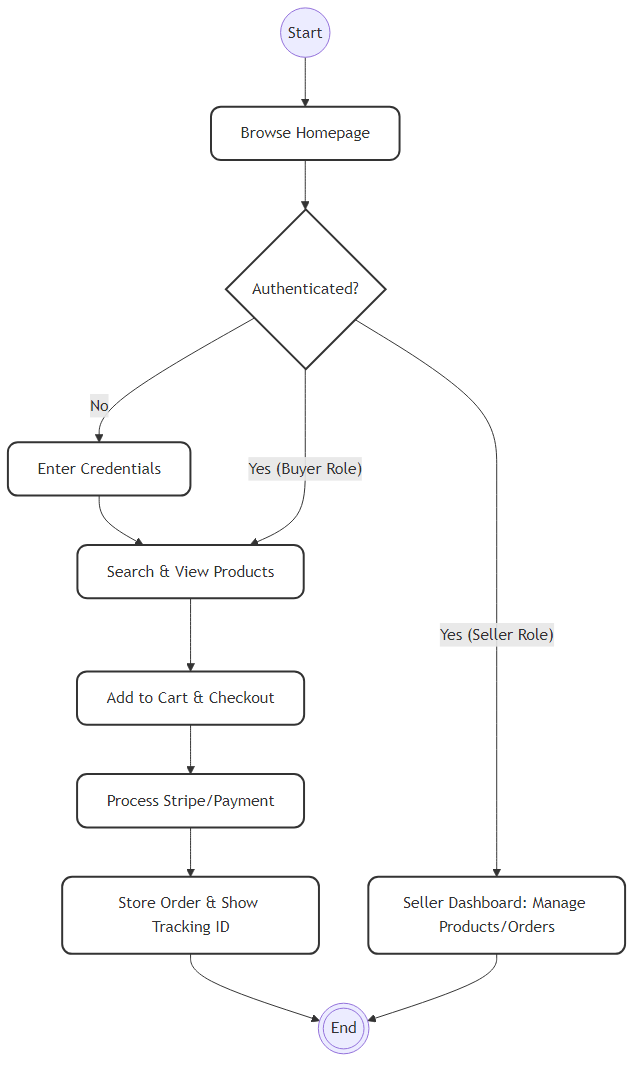
\includegraphics[width=0.8\textwidth]{activity_diagram.png}
    \caption{Shopify Activity Diagram}
    \label{fig:activity}
\end{figure}

\section{Database Schema \& Entities Design}
Unlike game development which might rely on localized JSON structs, Shopify utilizes a rigorous relational database design enforced through Laravel Migrations.
\begin{itemize}
    \item \textbf{Users Table:} Holds authentication and profile details, segmenting roles between general buyers and sellers.
    \item \textbf{Products Table:} Contains exhaustive product characteristics including pricing, seller relations, stock counts, and dynamic attributes.
    \item \textbf{Orders Table:} Tracks transaction states and fulfillment progress via a unique 10-character \texttt{tracking\_id}.
    \item \textbf{Embeddings Table:} A normalized structure dedicated to storing computed vector embeddings generated for semantic product similarity searches utilizing AI integrations.
\end{itemize}

\begin{figure}[H]
    \centering
    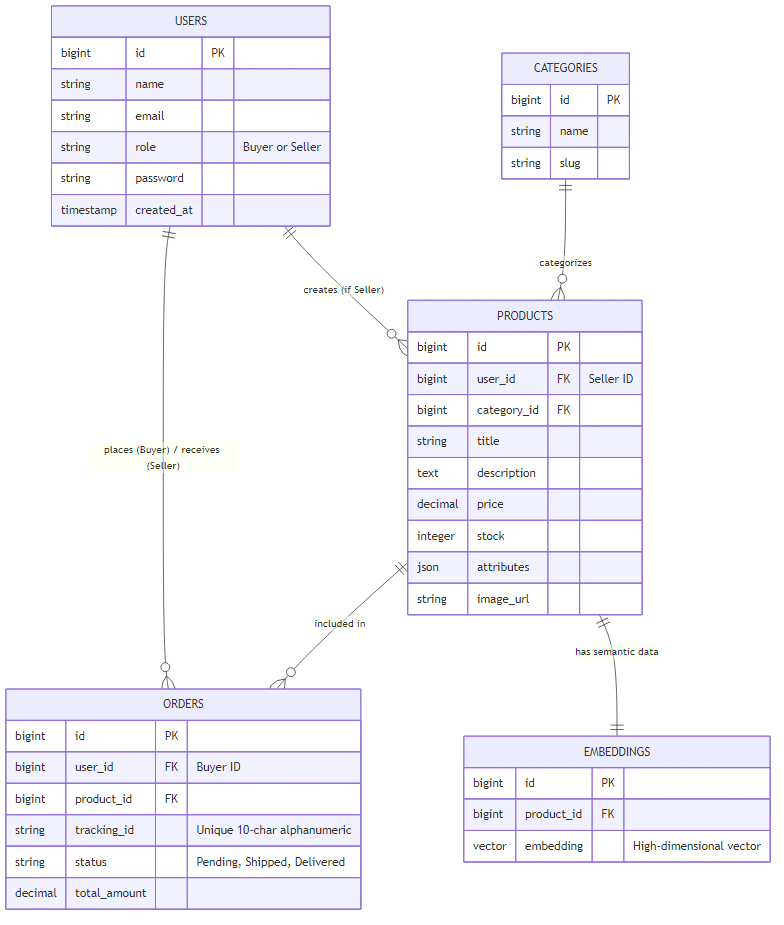
\includegraphics[width=0.8\textwidth]{er_diagram.png}
    \caption{Entity Relationship Diagram}
    \label{fig:er_diagram}
\end{figure}

\section{User Interface (UI) Design}
The interface components are modularly constructed in React, dynamically styled using Tailwind CSS to prioritize legibility, fast rendering, and clarity of action.

\begin{figure}[H]
    \centering
    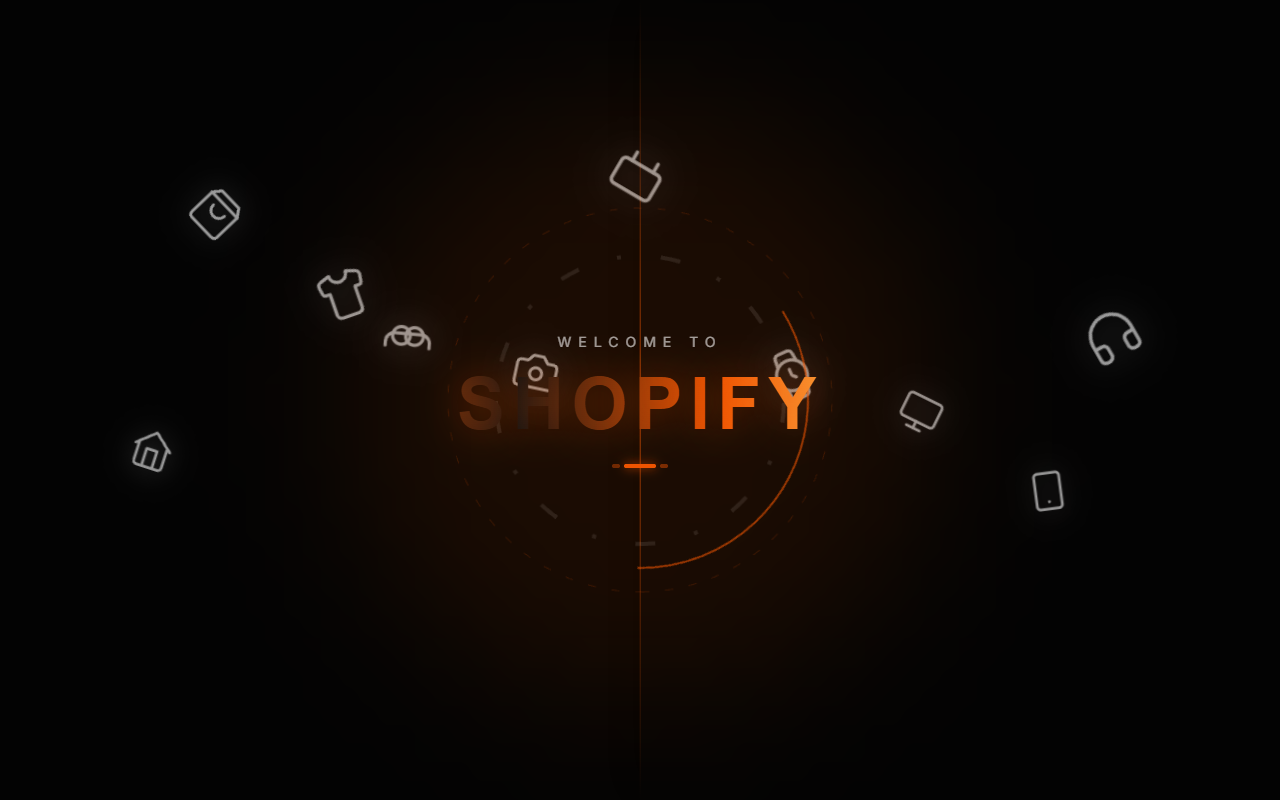
\includegraphics[width=0.8\textwidth]{home.png}
    \caption{Shopify Home Page Showcasing Product Catalog}
    \label{fig:home_ui}
\end{figure}

\textbf{Seller Dashboard UI:} Provides a secure, tabbed layout where sellers can observe aggregate stats, list new items with rich text descriptions, and quickly view which orders are pending dispatch.

\begin{figure}[H]
    \centering
    
\includegraphics[width=0.8\textwidth]{login.png}
    \caption{Secure Login Interface for Buyers and Sellers}
    \label{fig:login_ui}
\end{figure}
